\documentclass[tikz,border=5mm,12pt]{standalone}
\usepackage[fontsize=16pt]{fontsize}
\usetikzlibrary{arrows.meta}

\newcommand\myfbox[1]{\fbox{#1\strut}}

\def\labelYsep{32pt}
\def\xsep{56mm}
\def\ysep{14mm}
\begin{document}
  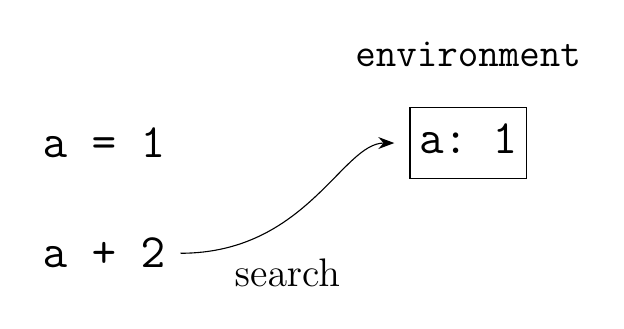
\begin{tikzpicture}[
    arrowtip/.style={
      -{Stealth[scale=1.2]}
    },
    upcurved/.style={
      in control={+(180:16mm)},
      out control={+(0:16mm)}
    },
    downcurved/.style={
      in control={+(180:4mm)},
      out control={+(-90:4mm)}
    },
    code/.style={
      anchor=west
    },
    subcode/.style={
      anchor=north west,below right=2mm
    }
  ]
    % left codes
    \node[code]       at (0*\xsep, 0*\ysep) { \texttt{a\ =\ 1} };
    \node[code] (OpB) at (0*\xsep,-1*\ysep) { \texttt{a\ +\ 2} };

    % right environments
    \node at (1*\xsep, \labelYsep) { \small\texttt{environment} };

    \node (EnvA) at (1*\xsep, 0*\ysep) { \myfbox{\texttt{a:\ 1}} };

    % arrows
    \draw[upcurved,arrowtip] (OpB.east)  to (EnvA);
    \path                    (OpB.east)  -- (EnvA) node[midway,below=4mm] { \small search };
  \end{tikzpicture}
\end{document}
